%% $RCSfile: proj_report_outline.tex,v $
%% $Revision: 1.2 $
%% $Date: 2010/04/23 02:40:16 $
%% $Author: kevin $

\documentclass[11pt
              , a4paper
              , twoside
              , openright
              ]{report}


\usepackage{float} % lets you have non-floating floats
\usepackage{graphicx}
\usepackage{url} % for typesetting urls
\usepackage{pdfpages}
%
%  We don't want figures to float so we define
%
\newfloat{fig}{thp}{lof}[chapter]
\floatname{fig}{Figure}

%% These are standard LaTeX definitions for the document
%%                            
\title{Milestone Report: Interactive 3D Visualisation of Exoplanets}
\author{Owen Bannister, 300172912}

%% This file can be used for creating a wide range of reports
%%  across various Schools
%%
%% Set up some things, mostly for the front page, for your specific document
%
% Current options are:
% [ecs|msor]              Which school you are in.
%
% [bschonscomp|mcompsci]  Which degree you are doing
%                          You can also specify any other degree by name
%                          (see below)
% [font|image]            Use a font or an image for the VUW logo
%                          The font option will only work on ECS systems
%
\usepackage[font,ecs,mcompsci]{vuwproject}

% You should specifiy your supervisor here with
     \supervisor{Stuart Marshall}
% use \supervisors if there is more than one supervisor

% Unless you've used the bschonscomp or mcompsci
%  options above use
   \otherdegree{Bachelor of Software Engineering with Honors}
% here to specify degree

% Comment this out if you want the date printed.
\date{}

\begin{document}

% Make the page numbering roman, until after the contents, etc.
\frontmatter

%%%%%%%%%%%%%%%%%%%%%%%%%%%%%%%%%%%%%%%%%%%%%%%%%%%%%%%

%%%%%%%%%%%%%%%%%%%%%%%%%%%%%%%%%%%%%%%%%%%%%%%%%%%%%%%

\begin{abstract}

We have lots of information about planets outside our solar system.
This can be accessed from a database by anyone. However this information is
complex and cannot be easily understood by a layperson. A visualisation will be
created for this information that can convey the information in a way lay people
can understand. The result of this project will be a visualisation system that can
be used as an information source for laypeople wanting to learn about planets
outside of the solar system. This report outlines the project, the progress that has been made, and the problems dealt with and solutions found.

\end{abstract}

%%%%%%%%%%%%%%%%%%%%%%%%%%%%%%%%%%%%%%%%%%%%%%%%%%%%%%%

\maketitle


\tableofcontents


%%%%%%%%%%%%%%%%%%%%%%%%%%%%%%%%%%%%%%%%%%%%%%%%%%%%%%%

\mainmatter

%%%%%%%%%%%%%%%%%%%%%%%%%%%%%%%%%%%%%%%%%%%%%%%%%%%%%%%

% individual chapters included here
\chapter{Introduction}
\section{Motivation}
There are many planets that have been located outside of our own solar system, these are called exoplanets. This project seeks to develop and evaluate an interactive 3D visualisation software system for the Kepler exoplanets dataset \cite{dataset}.  This visualisation will convey information in a way that the target users, laypeople who have an interest in astronomy, can understand.

\section{Problem Description}
Existing data visualisation techniques using this exoplanet dataset lack the ability to display
sufficient detail on each exoplanet and do not provide answers to questions that can be answered by the Exoplanet attributes in the dataset. Existing solutions use simple visualisations focusing on displaying
the planets in relation to their distance from their nearest star so that a proper sense of
scale to be perceived. Each candidate’s estimated size, orbital speed, and orbital separation
is accurately depicted, and each planet is color-coded according to its estimated effective
temperature.
\\\\
While this is a lot of information that can be used to inform users of important facts about
the planets, it does leave a lot of potential information undisplayed and overlooked. Currently only the size, temperature, and orbit sizes of Exoplanets have been displayed. This leaves a lot of information unseen, for example, information about the type of planet, planets with similar traits, solar system information, similarity to earth and habitability. This project will therefore be focused on researching, implementing, and evaluating a new
interactive visualisation system that will display additional information to users not included in previous visualisation systems.
\section{Proposed Solution}
The visualisation for this project will be created using Processing, a Java framework for visualisations. As the time is short for this project, I am extending a previous visualisation that uses the same dataset, the Kepler Visualisation Tool \cite{kepler_github, kepler_article}. The techniques that I will use to improve this visualisation will involve improving the methods of interaction that users can use with the system, as well as displaying more of the attributes of Exoplanets from the dataset in an informative visual way. 
\section{Variations from Project Proposal}
A variation in the current design of the system is that now emphasises small multiples and filtering of the Exoplanets to display the information more clearly to users. Instead of the visualisation only answering the 5 key questions as proposed in the proposal, the aim will now be displaying as much of the information in the dataset as possible without detracting from the effectiveness of the visualisation whilst still answering the questions. This is because the 5 questions did not fully utilize the information in the dataset. However I will need to ensure the effectiveness of the visualisation does not become diminished by trying to convey to much information which would lead to cluttering and overlapping in the visualisation, as well as information overload for users. There will also be larger emphasis placed on making the existing system more usable by improving the interaction methods for users. The following list outlines the new requirements for the visualisation being developed. This will be done by 
providing GUI elements for each form of interaction with the system, as well as ensuring all interaction methods are intuitive for users. 
\subsection{Changed Technology Requirements}
\begin{enumerate}
 \item It needs to have a low learning curve as the time available to learn a technology is small.
   \item It needs to be capable of 3D visualisations as it is more immersive to users.
   \item It needs to have prior evidence that it can be used to produce visualisations.
    \item It needs to allow user interaction with dynamic/animated transitions.
\end{enumerate}
\subsection{Changed Visualisation Requirements}
\begin{enumerate}
 \item All interaction methods must be visible and intuitive
 \item The visualisation needs to display answers to the 5 questions in the dataset
 \item The visualisation needs to display attributes of each of the Exoplanets
 \item The visualisation must remain uncluttered
 \item The visualisation must not show so much information that it caused information overload for users.
 \item Each Exoplanet must be selectable for further analysis
 \item Users need to be able to compare two selected Exoplanets
\end{enumerate}

\section{Contributions}
This project will provide an extension of the Kepler Visualisation Tool \cite{kepler_github} that conveys more information and is easier for users to interact with than the original. This extension will be evaluated by a user experiment to ensure that it is successful in conveying the information contained in the dataset.
\\\\
The work and research completed for this project will allow for further improvement by other developers and researchers to extend and improve the visualisation created. This will provide further exposure of the Kepler dataset which will encourage learning about Exoplanets.
\chapter{Prior Work}
\section{Literature Review}
\subsection{Layout of Multiple Views for Volume Visualization: A User Study}
Problems can occur when trying to organize many different views on one screen. However the different layout techniques
for multiple views evaluated resulted in no noticeable difference in user performance  \cite{lewis}.
\\\\
Typical volume visualization interface has a single rendering window and a
control panel that displays all the visualization parameters. Finding optimal settings
for the myriad of parameters by manipulating many individual controls can be overly
complicated and inefficient, and it can unnecessarily muddle the simplicity of a user’s
mental model of how an application works. Having too many individual controls
can reduce context and is unintuitive to users without expertise in graphics or
visualization \cite{lewis}. 
\\\\
This provides important insights into how the different windows for this visualisation should be layed out. Ensuring that the system is intuitive is important for the usability of the visualisation.
\subsection{A Survey on Multivariate Data Visualization}
However, extracting the meaningful information is a difficult task when large quantities of data are presented in plain text or traditional tabular form  \cite{chan}. Effective graphical representations of the data thus enjoy popularity by harnessing the human’s visual perception capabilities. Visualisations aim to help users to effectively detect and explore the expected, as well as discovering the unexpected to gain insight into the data. For multivariate data visualization, the dataset to be visually analyzed is of high dimensionality and these attributes are correlated in some way.
\\\\
This paper outlines many of the design techniques and tradeoffs that are used when creating visualisations for multivariate data. This will be useful as it provides insights into the effectiveness of different layouts of data.
\subsection{Exploratory Visualization of Multivariate Data with Variable Quality }
Real-world data is known to be imperfect, suffering from various forms of defects. An effective visualization system must make users aware of the quality of their data by explicitly conveying not only the actual data content, but also its quality attributes \cite{huang}.
\\\\
This is important for my project as the dataset I am using is made up from multiple releases from multiple years merged together to form a single dataset. This means that any errors in the data could cause the visualisation to display incorrect information. Using the ideas from this paper about displaying incorrect information will help to mitigate this. 
\subsection{Design Patterns for Rapid Visualization Prototyping}
This paper introduces three software design patterns
for rapid prototyping of information visualization applications \cite{ertl}.
The first pattern describes a mapping of object oriented
models to relational data tables used in many visualization
frameworks. The second pattern describes a script
based approach for the configuration of visualization applications.
The third pattern addresses the problem of performing
online changes on the visual mapping by enhancing
fine-grained mapping operators with scripting capabilities.
\\\\
This provides information on how to rapidly develop and prototype elements for my visualisation. Using knowledge from these patterns will encourage improved development times.
\subsection{Interactive Visualisation of a News Clips Network }
Finding a way for interactively exploring data through visualisation enables users to improve their understanding of provided information . They gain knowledge by "connecting the dots``, establishing mental relationships between individual pieces of data in an intuitive manor. The goal was to create an interface for users to explore already available information in a user friendly and insightful manor \cite{devezas}. 
\\\\
The interaction techniques of interest in this paper are, zooming, and pinning interesting elements for further analysis. A challenge they faced and solved was the identification of descriptive node labels, as well as their positioning .
\subsection{Position Statement Evaluating Information Visualizations: Issues and Opportunities}
It is still relatively common to see new information visualization techniques proposed that have high “wow” value: being visually striking and products of impressive technical engineering. Unfortunately, the potential value of many of these techniques in actually helping end-users solve problems and perform tasks is dubious in many cases \cite{stasko}. Evaluating information visualisation techniques and systems is important in order to understand how to improve them and to create innovative, useful new techniques. By better identifying the tasks that people perform using information visualisation tools as well as the insights gained within, one can conduct more rigorous and comprehensive assessments \cite{stasko}.
\\\\
While this paper is focused on creating and evaluation new visualisation techniques, it also provides insight into visualisations themselves. This is important for my visualisation as I will need to ensure that all visualisation techniques have the potential to help people and are not just “cool”. The information in this paper is important as it gives me many ways of carrying out, improving the evaluation of my visualisation as well as some of the challenges I will face.
\section{Visualisation Review}
Much of the research I have performed has been into other visualisations which focus on stars, space, or planets. I felt that these would be the most likely to offer insights into the techniques that I could use in my project.
\subsection{Worlds: The Kepler Planet Candidates - Non Interactive}
 This animation \cite{worlds} shows  planet candidates found by NASA's Kepler mission. These candidates are animated in orbit around a single star. They are drawn to scale with accurate radii, orbital periods, and orbital distances. They range in size from 1/3 to 84 times the radius of Earth. Colors represent an estimate of temperature with red indicating warmest, and blue indicating coldest candidates. 
\begin{figure}[h!]
  \centering
      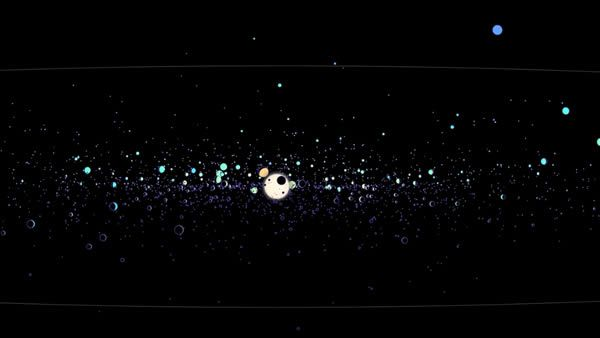
\includegraphics[width=0.8\textwidth]{images/worlds.jpg}
  \caption{Image of Worlds Visualisation}
\end{figure}
This animation is layed out very similarly to the Kepler Visualisation Tool that I am extending. This means that it provides insights into how my visualisation can be improved as Worlds is a much more visually appealing system. By researching how it displays its Exoplanets I can further improve my own visualisation.

\subsection{The Kepler Orrery and The Kepler Orrery 2 - Non interactive}
The Kepler Orrery \cite{orrery} illustrates the exoplanet candidates in their own solar systems. The orbit radii are to scale with respect to each other and planet sizes are to scale with respect to each other, but orbits and planet sizes are different scales. The colors are in order of semi-major axis: two-planet systems (242 in all) have a yellow outer planet; 3-planet (85) green, 4-planet (25) light blue, 5-planet (8) dark blue, 6-planet (1, Kepler-11) purple. 
\clearpage
\begin{figure}[h!]
  \centering
      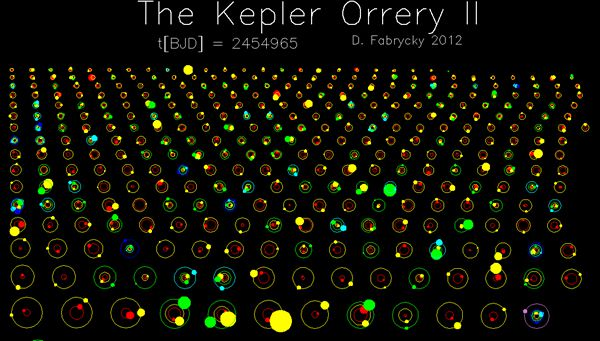
\includegraphics[width=0.8\textwidth]{images/orrery.jpg}
  \caption{Image of The Kepler Orrery Visualisation}
\end{figure}
This system exhibits small multiples, a grid of small similar graphics or charts, allowing them to be easily compared. This provides insights into how I can use small multiples to display information about groups of planets. This will be important for displaying which planets share a solar system.

\subsection{Celestia - Interactive}
Celestia \cite{celestia} is a free real-time space simulation that lets you visually experience the universe in three dimensions. It is an open source system written in C++. 
\begin{figure}[h!]
  \centering
      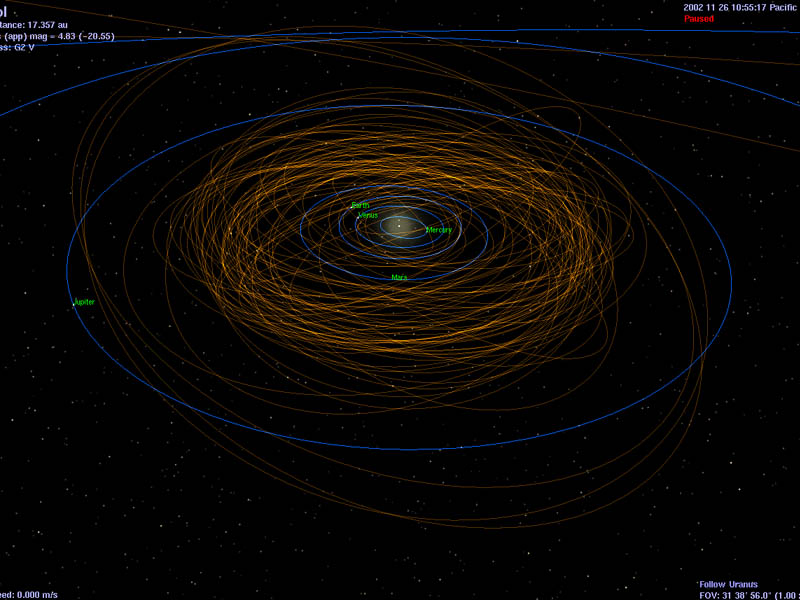
\includegraphics[width=0.5\textwidth]{images/celestia.jpg}
  \caption{Image of Celestia Visualisation}
\end{figure}
This visualisation is much larger and more encompassing system than is needed for this project, as it is a full 3D space simulation. However is does offer insights into how to effectively portray planets and their orbits (See Figure 2.3). It also provides textures that can be used in my visualisation to depict what planets actually look like to increase user immersion.

\subsection{Kepler Visualisation Tool}
An existing system built with Processing is the Kepler Visualisation Tool\cite{kepler_github, kepler_article}. It is a simple visualisation focusing on displaying the candidate Exoplanets temperatures and their locations in relation to their distance from their nearest star, so that a sense of scale can be perceived. Each candidate’s estimated size, orbital speed, and orbital separation is accurately depicted, and each planet is color-coded according to its estimated effective temperature.
\begin{figure}[h!]
  \centering
      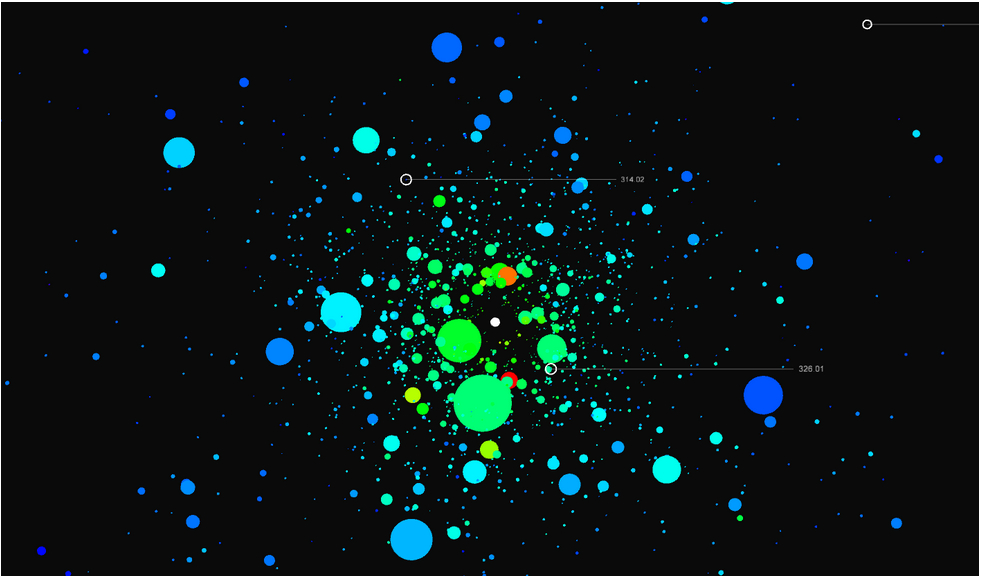
\includegraphics[width=0.8\textwidth]{images/kepler_orbital.jpg}
  \caption{Kepler Visualisation Tool Orbital View}
\end{figure}
\begin{figure}[h!]
  \centering
      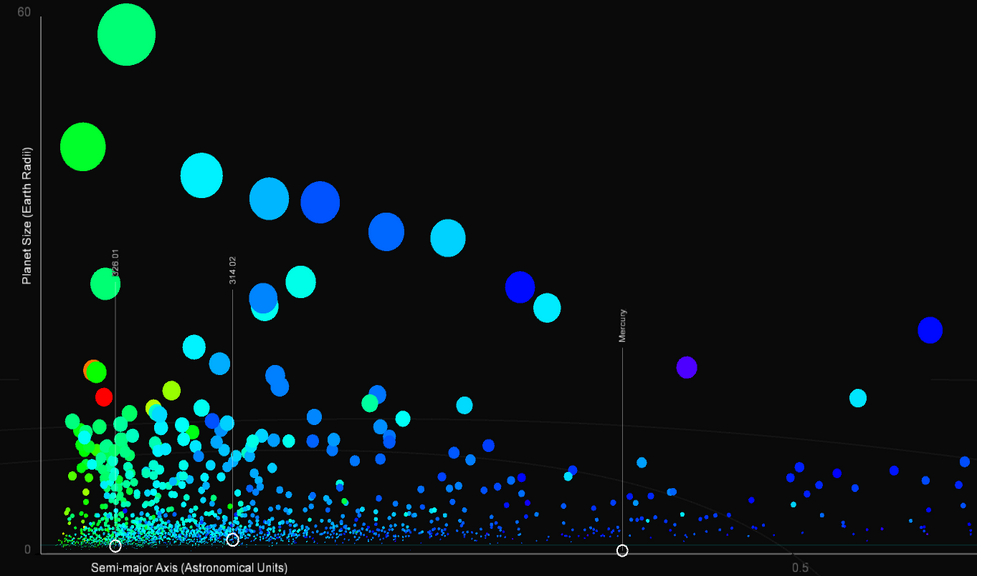
\includegraphics[width=0.8\textwidth]{images/kepler_graph.jpg}
  \caption{Kepler Visualisation Tool Graph View}
\end{figure}
The existing work in this system would serve as foundation for this project. Because much of the visual aspects, and initial data manipulation of the existing system are already complete. It means that implementing the features needed for this projects completion could be focused on more heavily and larger improvements to the existing system can be undertaken, such as better labeling and information displays and user interaction methods.

\chapter{Technology and Design}
\section{Choosing My Technology}
\subsection{Java using Swing or Processing}
Building a visualisation in Java would mean that I would be able to design it from the ground up. This would mean that there would be an almost non existent learning curve as I would not be extending an existing visualisation or learning a new technology.  If I were to use the GUI library Swing, it would involve using a drawing canvas or another graphic rendering tool. However by using this solution over tailored and  proven visualization toolkits I would be limiting the quality of the system. This is because the built in drawing methods in Java are primitive compared to some of the visualisation libraries and frameworks available.
\\\\
A better option would be to use Processing. Processing is an open source programming language and development environment that was initially created to serve as a software sketchbook and to teach the fundamentals of computer programming with a visual context. Using processing would mean that the visualization could be built with Java while still using a successful visualisation framework. The most complete existing visualization using the same exoplanet dataset (Kepler Visualization Tool) is built using Processing . 
\\\\
Using this solution would involve learning the Processing language, however Processing is a library built in Java so the syntax is the same. This means the learning curve in in regards to the program itself should be shallow.
\\\\
Using processing and would mean that 3D elements could be included, this wouldn’t be possible with D3. However it does require a strong knowledge in 3D transformations which I do not possess. This may be a limiting factor in the speed at which I could understand the existing code and may push using this solution out of scope in favor of D3.
\\\\
Two other technologies were researched before choosing processing, these were Prefuse, and D3.js (Appendix A.1). The Below table illustrates the reasons for choosing Processing.
\clearpage
\begin{figure}[h!]
  \centering
      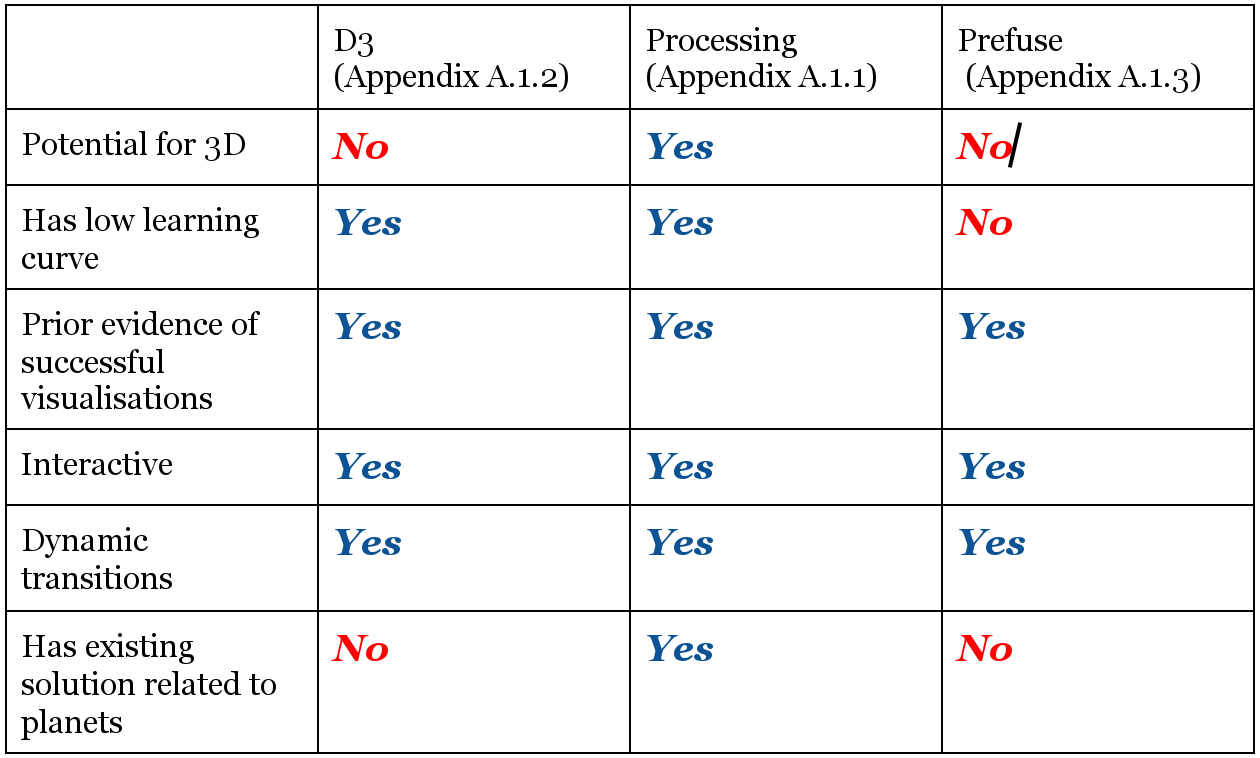
\includegraphics[width=0.8\textwidth]{images/table_technologies.jpg}
  \caption{Table of technology choices}
\end{figure}
Processing was chosen because of the advantages it had over the other technologies as shown in the table above. Although one of the strong advantages to Processing was that it has the previous visualisation that can be extended, this was only part of the reason for its choice. It also has a shallow learning curve as it uses Java as the programming language. I also only need to learn the required code needed for Processing, which the API and online examples make easy, as well having many opensource libraries available. Also the fact that it allows 3D animations and has strong interaction methods built into the language means that it was the most feasible choice of technology for this project.
\\\\
As well as using Processing as the tool for the visualisation, I will also extend the existing Kepler Visualization Tool. This is because it provides a basis for a visualisation as well as an initial design, and base functionality that will fast track my own development.

\section{Existing work on Kepler Visualization Tool \cite{kepler_article}}
The existing visualisation displays all Kepler candidates, arranged as if orbiting a single star. Each candidate's estimated size, orbital speed, and orbital separation is accurately depicted, and each planet is color-coded according to its estimated effective temperature, with red being relatively hot and deep blue/violet being relatively cold. Mercury, Mars, Earth, and Jupiter are added for context. Two concentric rings plot distances of 0.5 and 1 astronomical units from the central star, and a pale blue line delineates Earth's location on two self-organizing charts. In the video posted above, the first chart in the sequence plots semi-major axis (i.e., average orbital separation) versus effective temperature, while the second plots semi-major axis versus planetary size.
\\\\
The Kepler Visualisation Tool does a good job at displaying the size and temperature of planets. Important data trends emerge from this visualization. The abundance of smaller candidates and relative sparsity of larger ones clearly indicates that there are many tiny, meek worlds for every giant planet. The next 2 subsections detail the existing work done in this tool.
\subsection{Existing Layouts}
The existing visualisation has 2 different layouts for the data
\\\\
1. Orbital Layout - Shows exoplanets orbiting a single stars (Figure 3.2)
\\\\
2. Graph Layout - Used to display planets on x,y scale using attributes (Figure 3.3)

\subsection{Existing Interaction Techniques}
 The table below shows the interaction techniques in the existing system.
\\\\
\begin{figure}[h]
  \centering
      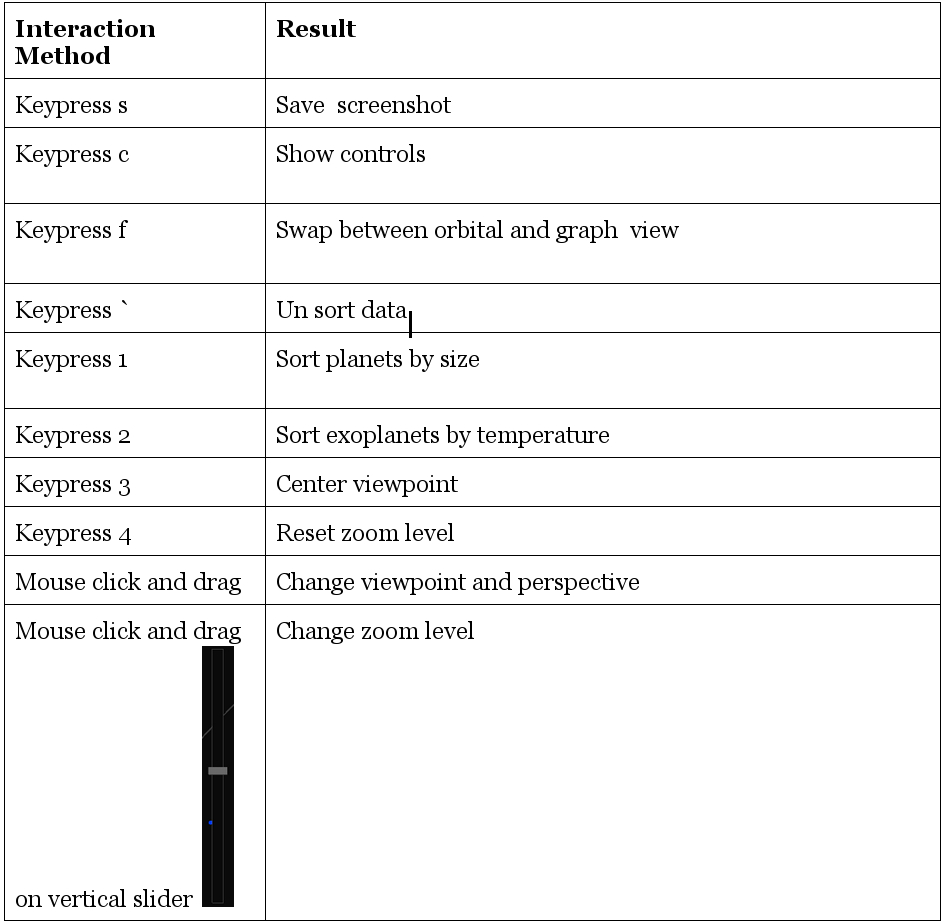
\includegraphics[width=0.8\textwidth]{images/table.jpg}
  \caption{Table of existing interaction methods in system}
\end{figure}

\chapter{Visualisation Design}
\section{Required User Interactions}
There are a set of interaction methods that are needed for this visualization. These interaction methods are needed to fulfill the visualisation requirements as outlined in section 1.4.2 These methods are:
\begin{enumerate}
 \item Select planets for further analysis.
 \item Select planet attribute to sort by.
 \item Allow non selected planets to be greyed out.
 \item Pause the orbit of planets to make selection easier.

\end{enumerate}
There are also improvements needed for the existing system to improve user interaction. This is because currently there is no visual indication of the interaction techniques. These improvements are:
\begin{enumerate}
 \item A panel containing buttons for each of the views changes
 \item Include scroll to zoom functionality
\end{enumerate}
\section{Layout Requirements}
By using abstract user interface design the layout and configuration of each element can be planned and coordinated without the need for excessive details which are likely to change throughout the course of the project (e.g., colours and content) \cite{martin}.
\\\\
The visualisation elements needed to convey the information in the dataset can be broken into 4 sections. This means that there should be a section in the layout of the visualization that corresponds to each. I have created 3 potential layouts and the optimal choice will be one that induces the lowest cognitive and load for users and is the most intuitive.  I am able to focus on creating a layout that does not create unneeded extraneous load \cite{InformationCapacity} on users. Doing this means that each section of the visualization needs to be separated spatially from one another so that the cognition needed to visually separate each section is minimal \cite{mendel}.  
\\\\
For this visualisation there is the need for 4 user interface boxes. 
\begin{enumerate}
\item Main Panel: Display the main visualisation. The other panels will be used to support this panel.
 \item Interaction Panel: Display the interaction components for the visualisation. This is because the existing solution has only key-presses as the way of modifying the visualisation. This is not sufficient as there is no indication in the system of how to use these. Also the proposed extensions to the system will require more advanced user interaction elements
\item Selected Planet Panel: Display the information about a selected planet.
\item Comparison Panel: Display a comparison between 2 selected elements.
\end{enumerate}
\begin{figure}[h!]
  \centering
      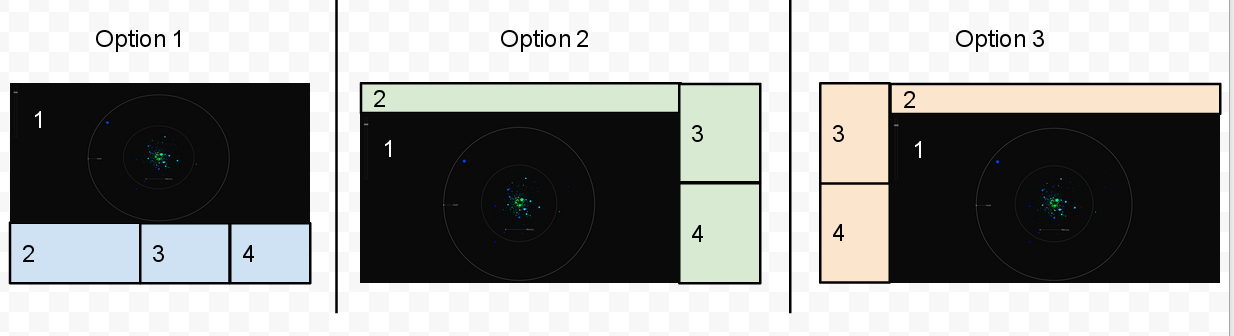
\includegraphics[width=0.8\textwidth]{images/layouts.jpg}
  \caption{Possible Layouts}
\end{figure}

These layouts will need to be evaluated to discover which is the most effective. It is possible that none of these options are suitable and the layout may need to be redesigned, however as the functionality will be implemented, changing the layout will be a trivial matter. 

\chapter{Progress}
\section{Progress Made}
The progress up to this point has been focused on researching and designing the layouts and methods of effectively displaying information about the Exoplanets. I have also made progress in modifying the existing code of the Kepler Visualisation Tool \cite{kepler_github} to make it easier to extend, as well as working on the ways that users can interact with the system. Due to the existing code being difficult to extend, my progress in implementing new features has been delayed. However I have still finished some key functionality for the visualisation.


\begin{figure}[h!]
  \centering
      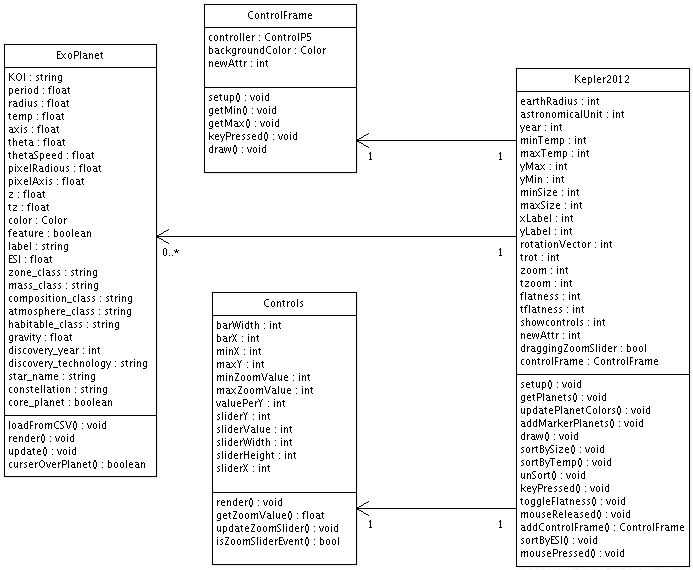
\includegraphics[width=0.8\textwidth]{images/KeplerVisualizationTool.png}
  \caption{Class Diagram of system}
\end{figure}
\begin{figure}[h!]
  \centering
      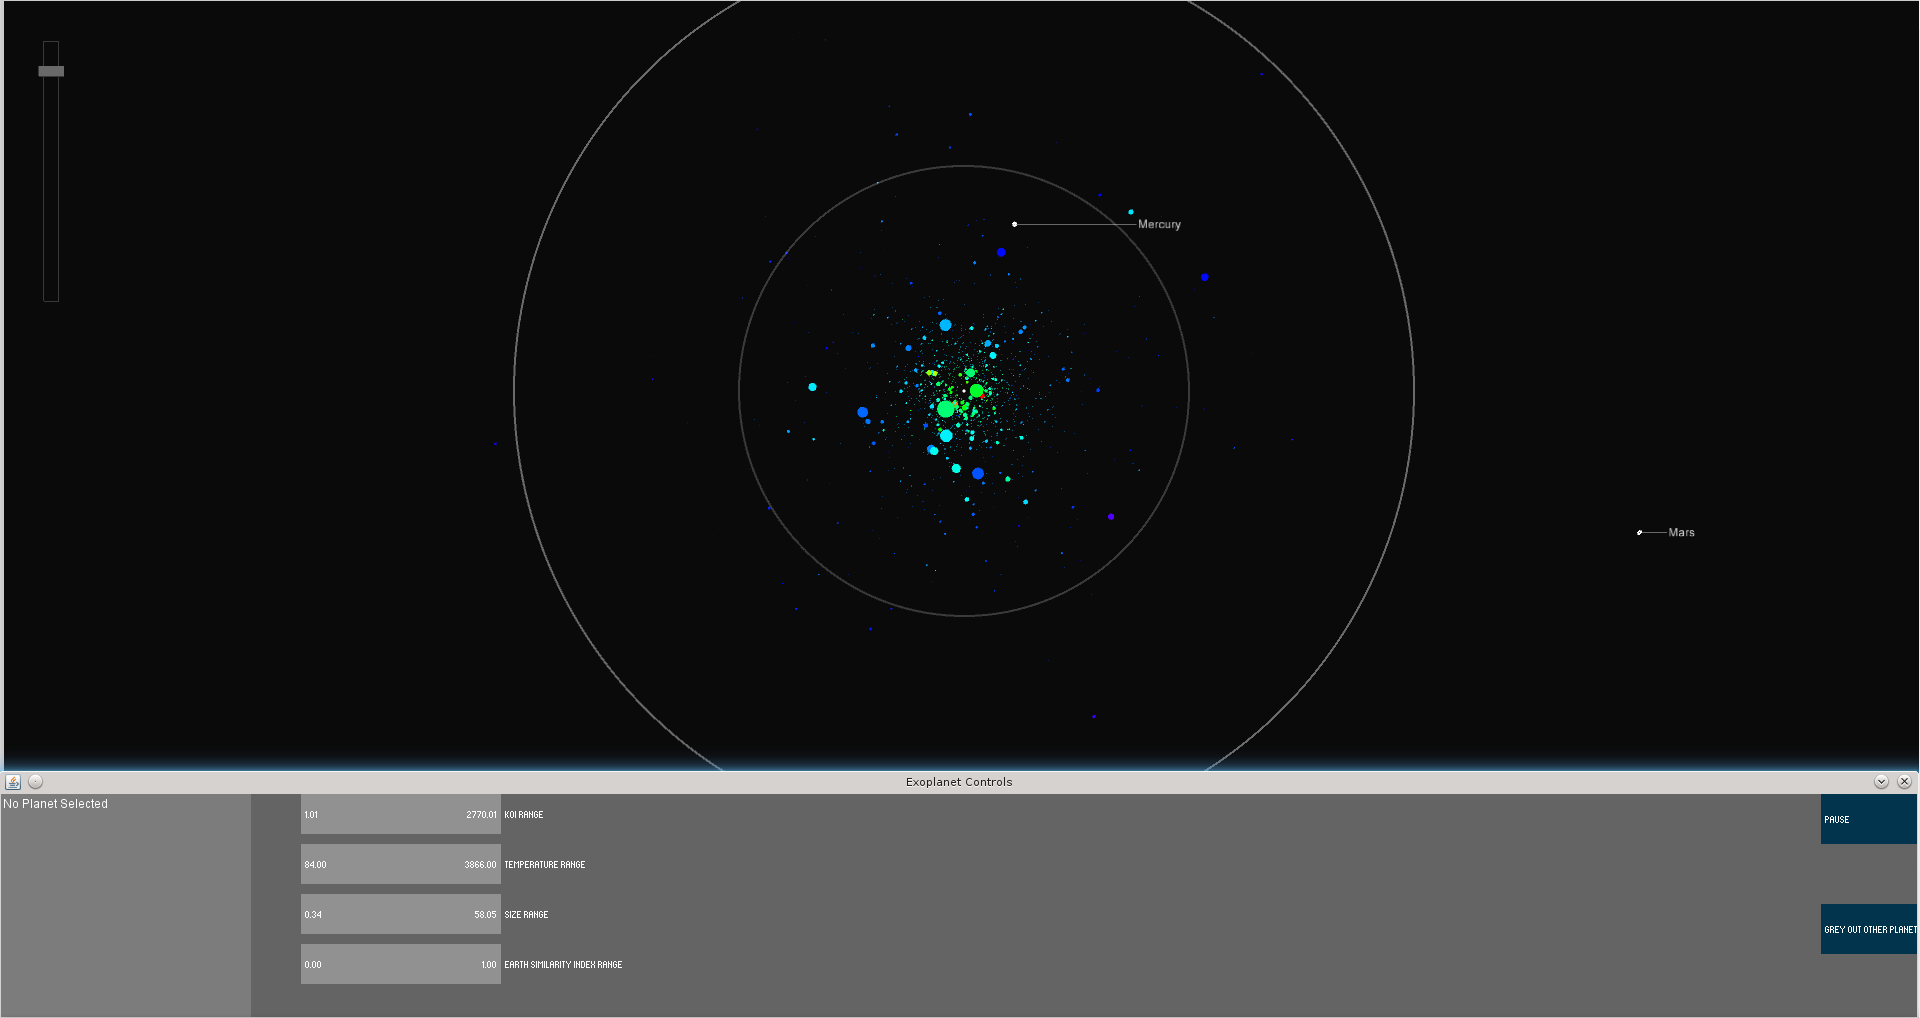
\includegraphics[width=0.8\textwidth]{images/system_so_far.jpg}
  \caption{Overview of Current System}
\end{figure}
I have implemented one new layout of the Exoplanet nodes in the graph to display their Earth Similarity Index following the mockup (Appendix A.2.3). Selection of planets has been implemented as before there was no way to interact with the Exoplanets in the visualisation. Also implemented is the interaction panel which allows the Exoplanets displayed to be filtered upon some of their attributes.Included in the panel is settings to allow planets from the same star system to be highlighted and all other greyed out as well as a button which allows pausing of the orbit of Exoplanets to make their selection easier. I have completed the filtering mechanism for the visualisation which allows users to specify the ranges of different attributes of the planets in order to view smaller subsets of Exoplanets.

\begin{figure}[h!]
  \centering
      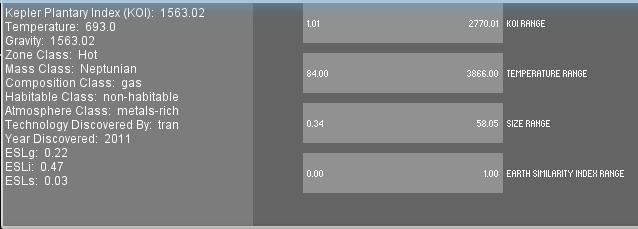
\includegraphics[width=0.8\textwidth]{images/interaction_panel.jpg}
  \caption{Interaction panel of system}
\end{figure}

\begin{figure}[h!]
  \centering
      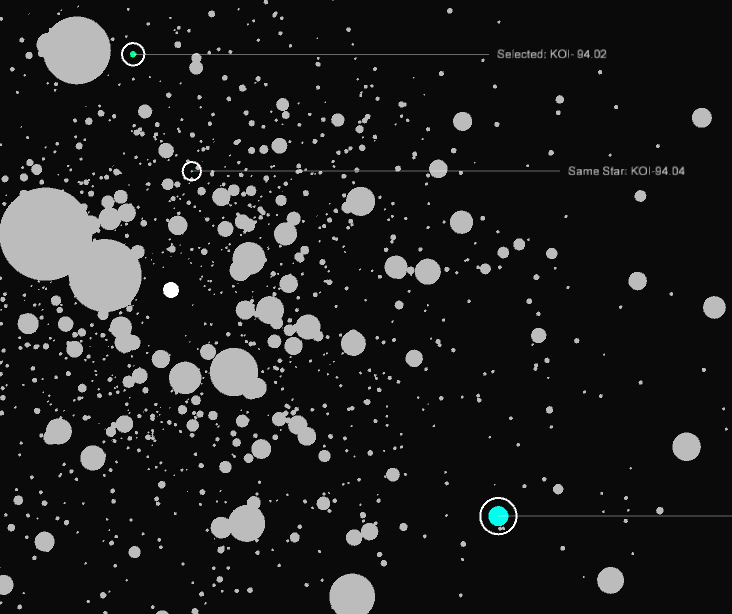
\includegraphics[width=0.8\textwidth]{images/greyed_out.jpg}
  \caption{Selected planets with all others grey}
\end{figure}
Much of my progress has been improving and customising the existing code so that I can extend it easily. This is because the existing system was built in a way that did not allow more than one variable of the Exoplanets to be used for placement position in the visualisation.
\section{Difficulties encountered with implementation}
Below are some of the problems I have faced while implementing the visualisation, some of these are still outstanding problems which still need to be addressed.
\\\\
Problem:\\
The existing solution was implemented in a way that only the z axis location of each exoplanet could be modified. This meant that to display multivariate data on more than one axis the method of translating planets needed to be modified.
\\\\
Solution:\\
I extended the existing draw method of planets where the x and y locations of exoplanets were set so that it can be changed. However there is still a problem that it does not animate this change, this will require modifying the method further to incrementally move the planets when the axis are modified.
\\\\
Problem:\\
Any on screen GUI elements were placed inside the visualisation on the same plane as the planets, and so are zoom-able as well as rotatable instead of being fixed as is needed for a GUI
\\\\
Solution:\\
I currently have a partial solution which is to use multiple frames for each window component. However this is not optimal as the main window needs to be selected for key presses to work even though it does allow the user to rearrange the different windows as they wish. 
\\\\
Problem: \\
Due to the large number of items to be displayed on screen there is a large amount of performance loss and sometimes crashes the visualisation due to an out of memory exception or simply freezing.
\\\\
Solution:\\
Filtering of data to reduce the amount of planets being rendered reduces this problem, but does not solve it. This is still an outstanding issue.
\\\\
Problem:\\
When filtering the exoplanets there is a lag in the rendering. 
\\\\
Solution:\\
I will find a more efficient way of sorting and filtering data. This is still an outstanding issue.
\\\\
Problem:\\
When a planet is selected and a button is clicked a NullPointerException is thrown
\\\\
Solution:\\
It was because the core planets of our solar system were being checked against due to them being considered feature planets when they should have been excluded. I refactored it so that they are now corePlanets and so the feature boolean can be used safely.
\chapter{Future Plans}
\section{Implementation}
The further implementation of the system will involve improving the interaction panel to improve user interactions. Further work will also go into how selected planets are viewed and compared against each other as well as a select by name method for planets. Also currently only one Exoplanet can be selected at a time, this will need to be extended to allow multiple selections. 
\\\\
Further design and implementation will need to be carried out for attributes in the dataset that are currently not visualised. I am carrying out this project using an iterative approach and designing, implementing, and evaluating a small amount of elements at a time.
\\\\
At this stage, the current elements in development are:
\begin{enumerate}
 \item Refine displaying Exoplanets in the same solar system
 \item View Exoplanets in the same constellation
 \item Create functionality to allow multiple stars to be selected for comparison
 \item Display a textured image of what each Exoplanet would look like
\end{enumerate}

\section{Evaluation}
The evaluation of this system will be based on a user study of the final visualisation design
chosen and implemented. The user study will need to be designed to evaluate whether this
system can effectively display the answers to the questions introduced previously and maintain
user interest. The evaluation would also focus on the users ability to efficiently navigate
through the 3D structure, and to accurately and precisely select exoplanets for further study,
and accurately and precisely manipulate filtering tools.The evaluation will be based on both
qualitative and quantitative analysis of users interaction with the system.
The evaluation will have 20 subjects, for a 10 minute evaluation. This timeframe is similar to
the amount of time that someone would spend at an information terminal in an observatory.
During the evaluation the users will be monitored either in person or by camera to evaluate
their experiences with the system.
\section{Report}
After the implementation and evaluation has been completed I will begin the report which I estimate will take approximately 60 hours.
\\\\
\begin{figure}[h!]
  \centering
      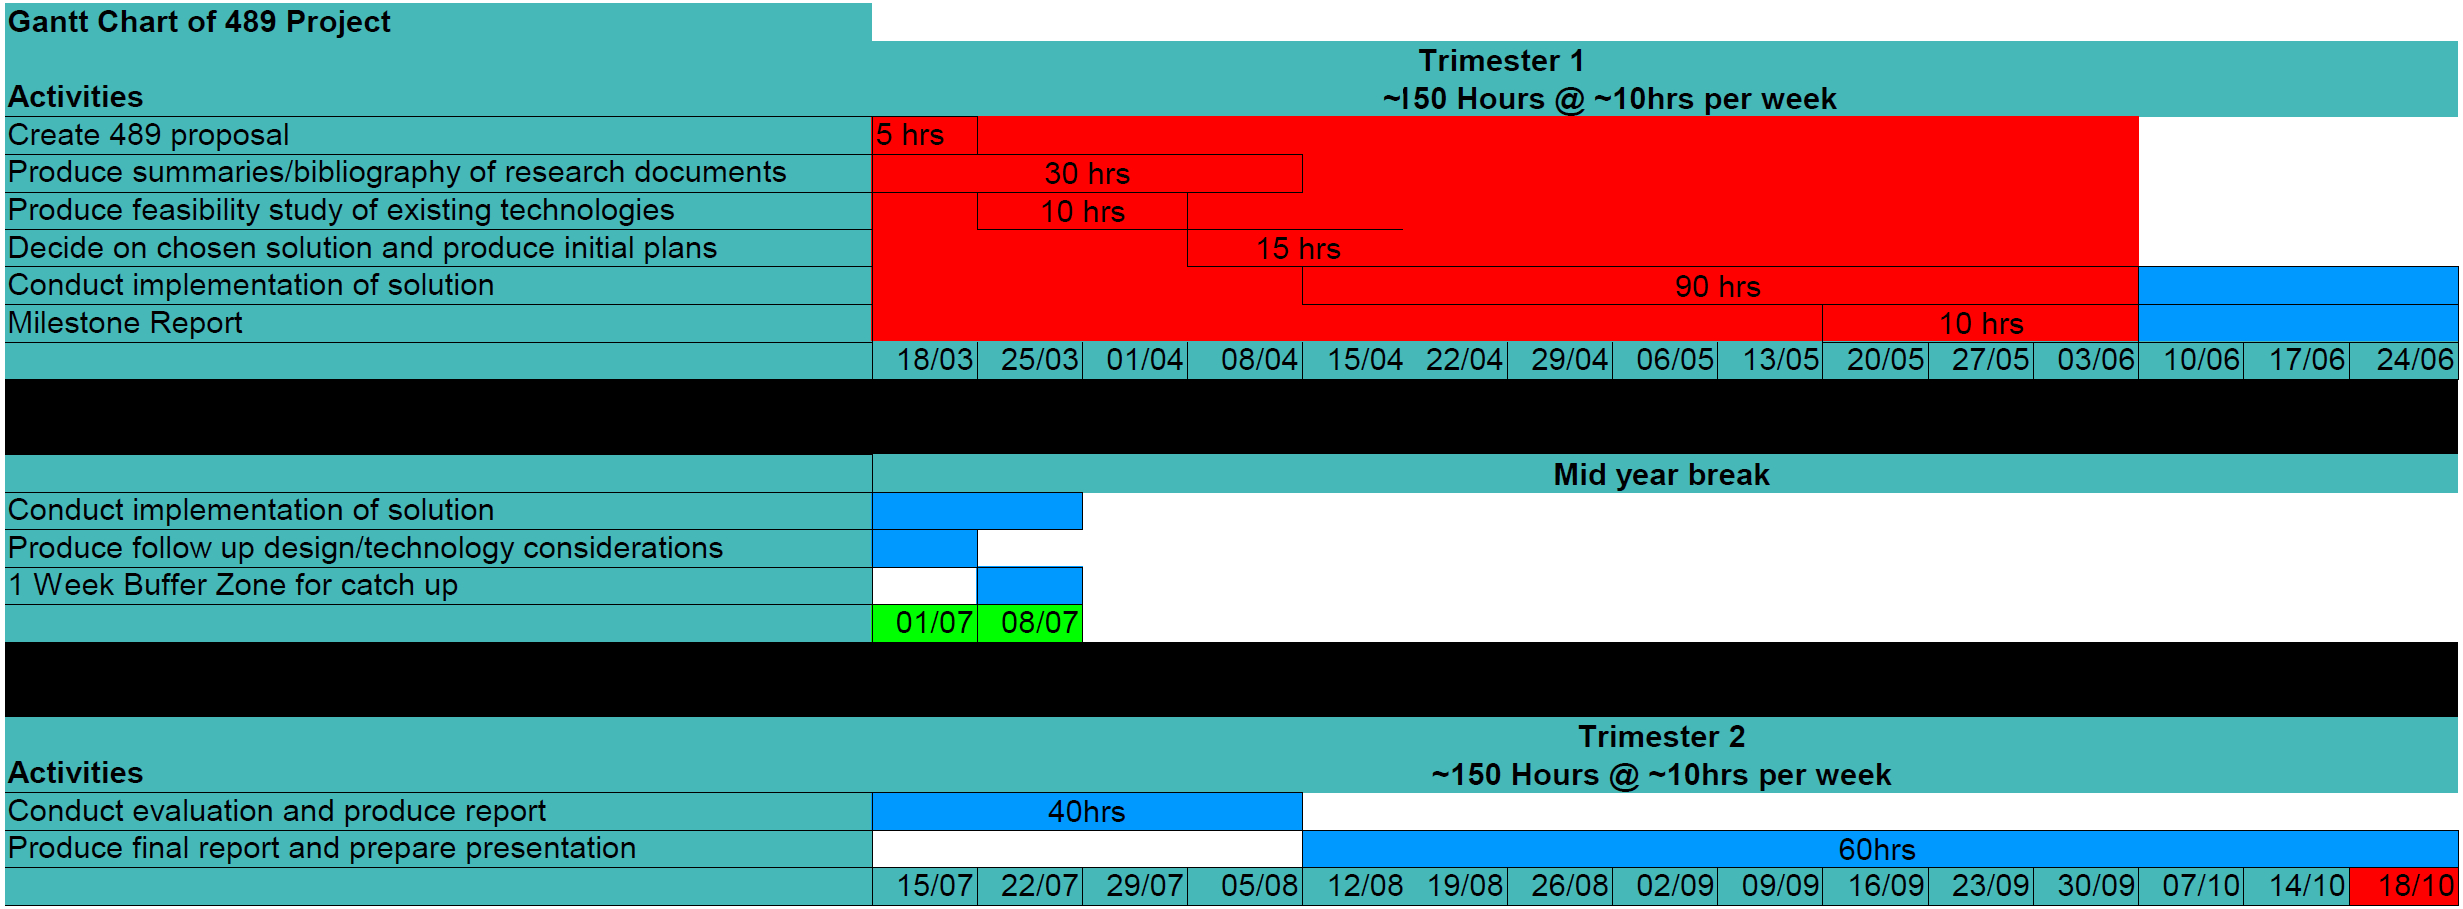
\includegraphics[width=1.5\textwidth,angle=90]{images/gantt_chart.jpg}
  \caption{Updated Gantt Chart}
\end{figure}
\chapter{Summary}
The report detailed the progress made on my project visualising Exoplanets discovered by the Kepler telescope. The progress made to this date has been made up of research, design, and implementation of my visualisation. The future plans involve further implementation and refinement of the visualisation. Followed by evaluation and write up.
%%%%%%%%%%%%%%%%%%%%%%%%%%%%%%%%%%%%%%%%%%%%%%%%%%%%%%%
\backmatter
%%%%%%%%%%%%%%%%%%%%%%%%%%%%%%%%%%%%%%%%%%%%%%%%%%%%%%%


%\bibliographystyle{ieeetr}
\nocite{*}
\bibliographystyle{acm}
\bibliography{sample}
\chapter{Appendix}
\section{Technology Option Exploration}

\subsection{D3 (Data-Driven Documents)}
D3 is a JavaScript library that allows the displaying of data in dynamic graphics. Embedded within an HTML web page, the JavaScript D3.js library uses pre-built JavaScript functions to select elements, create Scalable Vector Graphic (SVG)\cite{svg} objects, style them, and add transitions, dynamic effects and tooltips. Large datasets can be easily bound to SVG objects using simple D3 functions to generate rich charts and diagrams. D3 was created because of the need for a balance of expressiveness, efficiency, and accessibility that previous visualization toolkits did not allow \cite{d3}. 
\\\\
D3 allows the binding of input data to arbitrary input elements. This means that the exoplanet dataset can easily be bound to SVG elements for creating visualizations. D3 adopts the W3C Selectors API to identify document elements queried. This results in a rich but concise selection method of elements in a visualisation. 
\\\\
D3 allows debugging thanks to Google chrome and other modern browsers development tools. A downside to D3 is that it does not allow 3D diagrams, although it does allow pseudo 3D by using the painter's algorithm and textures.
\\\\
\begin{figure}[h!]
  \centering
      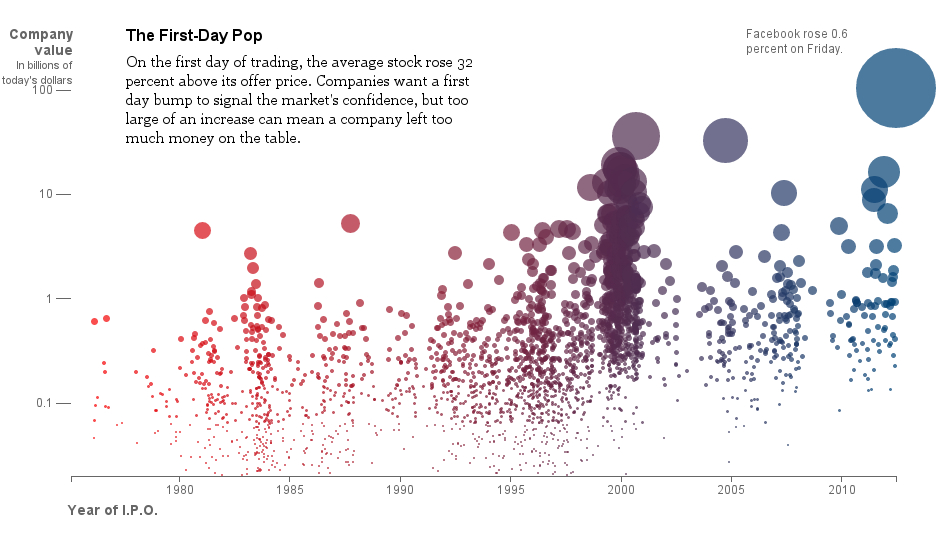
\includegraphics[width=0.8\textwidth]{images/d31.jpg}
  \caption{Example system in D3 showing Facebook statistics \cite{d3example}}
\end{figure}
\subsection{Prefuse}
Prefuse is a set of software tools for creating rich interactive data visualizations \cite{prefuse}. The Prefuse toolkit provides a visualization framework for Java.  It supports a set of features for visualizing and interacting with data. It provides optimized data structures for tables, graphs, and trees. It can be used to build standalone applications, visual components embedded in larger applications, and web applets. Prefuse to greatly simplifies the process of representing and efficiently handling data, mapping data to visual representations (e.g., through spatial position, size, shape, color, etc), and interacting with the data. 
\\\\
To use Prefuse a basic familiarity with the Java is required, including setting up and building Java projects. A knowledge of Swing or another similar user interface toolkit is also useful for understanding some of the concepts behind Prefuse and for integrating Prefuse visualizations into larger applications. Experience with database systems is also helpful.
\\\\
However the complexity of Prefuse means that the learning curve will be out of scope for this project. 
\section{Screen Mockups}
\subsection{Screen Mockup: Visualisation Interaction Panel(Panel 1)}

\begin{figure}[h!]
  \centering
      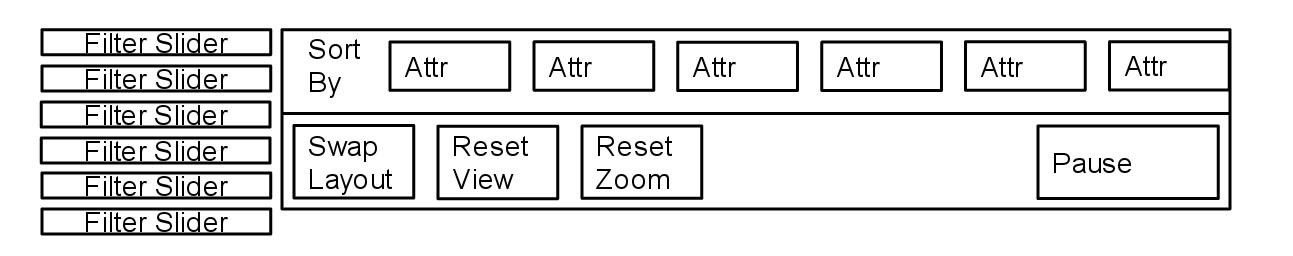
\includegraphics[width=0.8\textwidth]{images/interaction_mock.jpg}
  \caption{Mockup of interaction panel}
\end{figure}

By keeping the most widely used interaction elements at the edges of the visualisation it will allow mouse flicking for efficient component selection. Also by allowing GUI interactive elements as well as maintaining the existing key press interactivity it should allow a good balance between advanced and novice users. To improve this, each of the on screen interactive elements will also depict the keystroke that yields the same functionality as a way of transitioning novice users to advanced.

\subsection{Screen Mockup: Selected Planet Panel (Panel 2)}
\begin{figure}[h!]
  \centering
      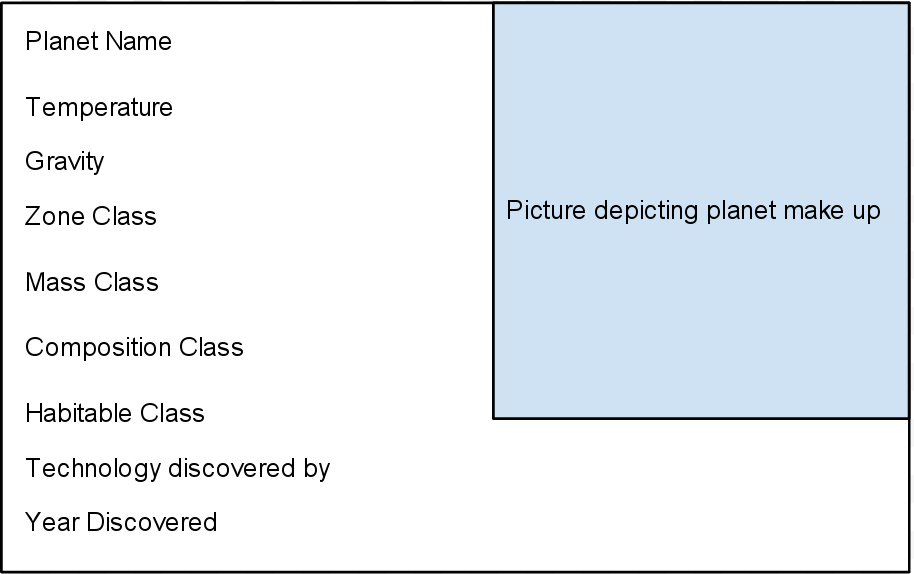
\includegraphics[width=0.8\textwidth]{images/planet_mock.jpg}
  \caption{Mockup of planet information panel}
\end{figure}

Explanation:
Using the vertical placement of Exoplanets to display their ESI while maintaining their horizontal placement should aid in comprehension by users about the comparisons to Earth
\subsection{Screen Mockup: Main panel (Panel 4)}
\subsubsection{Earth Similarity Index (ESIs, ESIi, ESIg) }
\begin{figure}[h!]
  \centering
      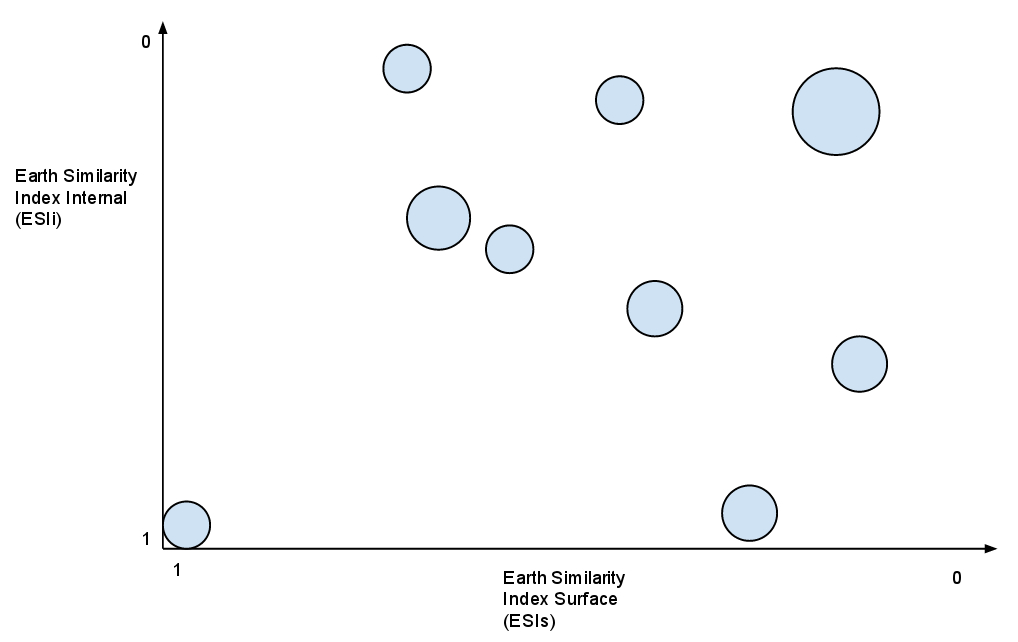
\includegraphics[width=0.8\textwidth]{images/esi_mock.jpg}
  \caption{Mockup of planet ESI view in graph layout}
\end{figure}
Explanation:\\
Using the vertical placement of Exoplants to display their ESI while maintaining their horizontal placement should aid in comprehension by users about the comparisons to Earth
\\\\
Placement:\\
Exoplanets\\
Vertical Alignment = ESIg\\
Horizontal Alignment = Semi-Major-Axis(AU)
\\\\
Earth\\
Vertical Alignment = 1.0 ESIg\\
Horizontal Alignment = Center of exoplanet orbit
\\\\
Star\\
Vertical Alignment = 0.0 ESIg\\
Horizontal Alignment =  Center of exoplanet orbit
\end{document}
